\documentclass[tikz]{standalone}
\usepackage{amsmath,amssymb}
\usepackage{pgfplots,multicol}

\pgfplotsset{compat=1.10}
\usepgfplotslibrary{fillbetween}

\begin{document}



 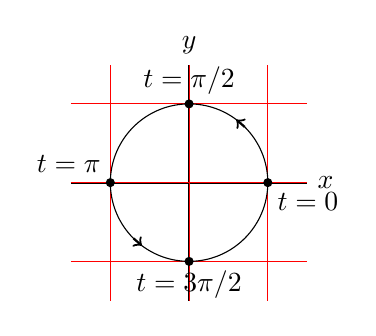
\begin{tikzpicture}[]
        \draw[-,thick] (-1.5,0) -- (1.5,0) node[right] {$x$};
         \draw[-,thick] (0,-1.5) -- (0,1.5) node[above] {$y$};
\draw[step=1.0,red,thin] (-1.5,-1.5) grid (1.5,1.5);
%	\foreach \x in {-4,-2,2,4,6}
%	 \draw[-,thick] (\x,0.1) -- (\x,-0.1) node[below] {\x};
%	 
%	 	\foreach \y in {-4,-2,2,4,6}
%	 \draw[-,thick] (0.1,\y) -- (-0.1,\y) node[left] {\y};
	
	
\draw[fill=black] (0,1) circle (0.05cm) node[above] {$t=\pi/2$};
\draw[fill=black] (-1,0) circle (0.05cm) node[above left] {$t=\pi$};
\draw[fill=black] (0,-1) circle (0.05cm) node[below] {$t=3\pi/2$};
\draw[fill=black] (1,0) circle (0.05cm) node[below right] {$t=0$};

\draw[] (0,0) circle (1);

\draw[->,thick] (0.707,0.707) -- (0.6,0.8) node[above] {};

\draw[->,thick] (-0.707,-0.707) -- (-0.6,-0.8) node[above] {};

\end{tikzpicture}


	
\end{document}
